\documentclass[11pt,a4paper]{article}
\usepackage{fontspec}
\setmainfont{Times New Roman}
\setsansfont{Arial}
\setmonofont{Consolas}
\usepackage[a4paper,margin=2.0cm]{geometry}
\usepackage{xcolor}
\usepackage{tikz}
\usetikzlibrary{calc}
\usepackage{booktabs}
\usepackage{tabularx}
\usepackage{graphicx}
\usepackage{float}
\usepackage{listings}
\usepackage{hyperref}
\usepackage{fancyhdr}

\definecolor{deepblue}{RGB}{14,58,130}
\definecolor{accentblue}{RGB}{37,99,235}
\definecolor{codebg}{RGB}{247,249,252}

\setlength{\emergencystretch}{3em}
\hbadness=10000
\hfuzz=2pt

\lstdefinelanguage{SystemVerilog}{
    keywords={module,endmodule,input,output,inout,logic,signed,parameter,localparam,typedef,enum,always_ff,always_comb,posedge,negedge,or,if,else,case,endcase,default,begin,end,for,integer},
    sensitive=true,
    morecomment=[l]{//},
    morecomment=[s]{/*}{*/}
}

\lstset{
    language=SystemVerilog,
    backgroundcolor=\color{codebg},
    basicstyle=\ttfamily\scriptsize,
    keywordstyle=\color{deepblue}\bfseries,
    commentstyle=\color{gray}\itshape,
    frame=single,
    rulecolor=\color{accentblue!40},
    breaklines=true,
    breakatwhitespace=false,
    columns=fullflexible,
    keepspaces=true,
    showstringspaces=false,
    tabsize=4
}

\pagestyle{fancy}
\fancyhf{}
\fancyhead[L]{\small\textcolor{deepblue}{Báo Cáo Thực Hành Thiết Kế Số \& FPGA Autopilot}}
\fancyhead[R]{\small\texttt{traffic\_fsm}}
\fancyfoot[C]{\thepage}

\begin{document}

% ==================== TIKZ BLUE DOUBLE-LINE COVER PAGE ====================
\begin{titlepage}
    \begin{tikzpicture}[remember picture, overlay]
        \draw[color=deepblue, line width=2.4pt]
            ($(current page.north west)+(1.2cm,-1.2cm)$)
            rectangle
            ($(current page.south east)+(-1.2cm,1.2cm)$);
        \draw[color=accentblue, line width=0.9pt]
            ($(current page.north west)+(1.42cm,-1.42cm)$)
            rectangle
            ($(current page.south east)+(-1.42cm,1.42cm)$);
    \end{tikzpicture}

    \centering
    \vspace*{1.6cm}
    {\Large\bfseries\textcolor{deepblue}{ĐẠI HỌC QUỐC GIA — PHÒNG THÍ NGHIỆM VI MẠCH \& FPGA}\\[0.3cm]}
    {\large\textsc{Digital Systems Design \& Quartus II Verification Lab Report}}\\[1.2cm]

    \rule{0.82\textwidth}{1.2pt}\\[0.5cm]
    {\huge\bfseries\textcolor{deepblue}{Parameterized Clock Divider + Smart Traffic Light Moore FSM}}\\[0.4cm]
    {\Large Module: \texttt{traffic\_fsm}}\\[0.4cm]
    \rule{0.82\textwidth}{1.2pt}\\[1.4cm]

    \begin{tabularx}{0.84\textwidth}{@{}lX@{}}
        \toprule
        \textbf{Hạng mục (Metadata)} & \textbf{Thông số kỹ thuật (Specification)} \\
        \midrule
        Tên bài thí nghiệm (Benchmark) & \texttt{traffic\_fsm} \\
        Kit FPGA mục tiêu (Target Kit) & DE2-115 (Cyclone IV E) \\
        Mã chip FPGA (Device Part) & \texttt{EP4CE115F29C7} \\
        Tần số xung nhịp (Target Clock) & 50.0 MHz \\
        Kết quả kiểm tra tĩnh (Static Lint) & PASS (0 Latches, 0 Width Warnings) \\
        Kết quả mô phỏng (Self-Checking TB) & 230 / 230 Vectors Passed (100\%) \\
        Trình tổng hợp (Synthesis Engine) & \texttt{quartus} \\
        \bottomrule
    \end{tabularx}

    \vfill
    {\normalsize Hệ thống tự động hóa thiết kế và kiểm chứng phần cứng \textbf{FPGA Autopilot}}\\[0.2cm]
    {\small Generated with 100\% Bit-Exact Simulation \& Hardware Synthesis Verification}
    \vspace*{1.2cm}
\end{titlepage}

\section{Tổng Quan Thiết Kế \& Đặc Tả Cổng Giao Tiếp (Port Specification)}
Synchronous smart intersection controller featuring a parameterized 50 MHz / SIM\_MODE 1-Hz tick divider, 2-FF asynchronous input synchronizer and counter debouncer for pedestrian button requests, emergency all-red override, countdown display, and glitch-free Moore traffic outputs.

\begin{table}[H]
    \centering
    \small
    \caption{Bảng đặc tả giao diện cổng vào/ra của module \texttt{traffic\_fsm}}
    \begin{tabularx}{\textwidth}{@{}llllX@{}}
        \toprule
        \textbf{Port} & \textbf{Dir} & \textbf{Width} & \textbf{Type} & \textbf{Chức năng (Description)} \\
        \midrule
        \texttt{clk} & input & 1 & logic & 50 MHz system clock \\
        \texttt{rst\_n} & input & 1 & active-low & Asynchronous active-low system reset \\
        \texttt{ped\_btn\_raw} & input & 1 & logic & Asynchronous pedestrian request push-button \\
        \texttt{emergency\_ovr} & input & 1 & logic & Synchronous high-priority emergency all-red override \\
        \texttt{ns\_light} & output & 3 & logic & North-South \{Red, Yellow, Green\} one-hot lamp bus \\
        \texttt{ew\_light} & output & 3 & logic & East-West \{Red, Yellow, Green\} one-hot lamp bus \\
        \texttt{ped\_walk} & output & 1 & logic & Pedestrian WALK indicator \\
        \texttt{countdown} & output & 4 & logic & Remaining seconds in active phase \\
        \bottomrule
    \end{tabularx}
\end{table}

\section{Finite State Machine Transition Table}
\begin{table}[H]
    \centering
    \small
    \caption{Synchronous Moore FSM State Encoding and Transitions}
    \begin{tabularx}{\textwidth}{@{}llXX@{}}
        \toprule
        \textbf{State} & \textbf{Code} & \textbf{Moore Outputs} & \textbf{Transition Condition} \\
        \midrule
        \texttt{ST\_NS\_GREEN} & 3'd0 & ns\_light=GREEN (001), ew\_light=RED (100), ped\_walk=0 & emergency\_ovr -> ST\_EMERGENCY; phase\_done -> ST\_NS\_YELLOW \\
        \texttt{ST\_NS\_YELLOW} & 3'd1 & ns\_light=YELLOW (010), ew\_light=RED (100), ped\_walk=0 & emergency\_ovr -> ST\_EMERGENCY; phase\_done -> ST\_ALL\_RED\_1 \\
        \texttt{ST\_ALL\_RED\_1} & 3'd2 & ns\_light=RED (100), ew\_light=RED (100), ped\_walk=0 & phase\_done \& ped\_pending -> ST\_PED\_WALK; phase\_done \& !ped\_pending -> ST\_EW\_GREEN \\
        \texttt{ST\_EW\_GREEN} & 3'd3 & ns\_light=RED (100), ew\_light=GREEN (001), ped\_walk=0 & emergency\_ovr -> ST\_EMERGENCY; phase\_done -> ST\_EW\_YELLOW \\
        \texttt{ST\_EW\_YELLOW} & 3'd4 & ns\_light=RED (100), ew\_light=YELLOW (010), ped\_walk=0 & emergency\_ovr -> ST\_EMERGENCY; phase\_done -> ST\_ALL\_RED\_2 \\
        \texttt{ST\_ALL\_RED\_2} & 3'd5 & ns\_light=RED (100), ew\_light=RED (100), ped\_walk=0 & phase\_done \& ped\_pending -> ST\_PED\_WALK; phase\_done \& !ped\_pending -> ST\_NS\_GREEN \\
        \texttt{ST\_PED\_WALK} & 3'd6 & ns\_light=RED (100), ew\_light=RED (100), ped\_walk=1 & phase\_done \& resume\_to\_ew -> ST\_EW\_GREEN; phase\_done \& !resume\_to\_ew -> ST\_NS\_GREEN \\
        \texttt{ST\_EMERGENCY} & 3'd7 & ns\_light=RED (100), ew\_light=RED (100), ped\_walk=0 & !emergency\_ovr -> ST\_ALL\_RED\_1 \\
        \bottomrule
    \end{tabularx}
\end{table}


\section{Triển Khai RTL SystemVerilog Chuẩn Tổng Hợp (Synthesizable RTL)}
Thiết kế tuân thủ nghiêm ngặt quy tắc SystemVerilog-2012: sử dụng \texttt{always\_ff} với phép gán không chặn (\texttt{<=}) cho mạch tuần tự, \texttt{always\_comb} với giá trị mặc định tường minh ở đầu khối cho mạch tổ hợp, cam kết \textbf{0 inferred latches}.

\begin{lstlisting}
// Auto-generated by fpga_autopilot — Strict Synthesizable SystemVerilog-2012
// Parameterized tick divider + 2-FF synchronizer + debouncer + Moore Traffic FSM

module traffic_fsm #(
    parameter [31:0] SIM_MODE          = 32'd0,
    parameter [31:0] CLK_FREQ_HZ       = 32'd50000000,
    parameter [31:0] SIM_TICKS_PER_SEC = 32'd4,
    parameter [3:0]  GREEN_SEC         = 4'd6,
    parameter [3:0]  YELLOW_SEC        = 4'd2,
    parameter [3:0]  PED_SEC           = 4'd4,
    parameter [3:0]  ALL_RED_SEC       = 4'd1
) (
    input  logic       clk,
    input  logic       rst_n,
    input  logic       ped_btn_raw,
    input  logic       emergency_ovr,
    output logic [2:0] ns_light,
    output logic [2:0] ew_light,
    output logic       ped_walk,
    output logic [3:0] countdown
);

    typedef enum logic [2:0] {
        ST_NS_GREEN  = 3'd0,
        ST_NS_YELLOW = 3'd1,
        ST_ALL_RED_1 = 3'd2,
        ST_EW_GREEN  = 3'd3,
        ST_EW_YELLOW = 3'd4,
        ST_ALL_RED_2 = 3'd5,
        ST_PED_WALK  = 3'd6,
        ST_EMERGENCY = 3'd7
    } state_t;

    localparam [31:0] TICKS_PER_SEC = (SIM_MODE != 32'd0) ? SIM_TICKS_PER_SEC : CLK_FREQ_HZ;
    localparam [31:0] DEBOUNCE_MAX  = (SIM_MODE != 32'd0) ? 32'd2 : (CLK_FREQ_HZ / 32'd100);

    localparam [2:0] LIGHT_RED    = 3'b100;
    localparam [2:0] LIGHT_YELLOW = 3'b010;
    localparam [2:0] LIGHT_GREEN  = 3'b001;

    state_t      state, next_state;
    logic [31:0] tick_cnt;
    logic        sec_tick;
    logic        phase_done;
    logic [3:0]  timer_sec;
    logic [3:0]  next_duration;

    // 2-FF synchronizer + debouncer for asynchronous pedestrian button
    logic        ped_sync_ff1;
    logic        ped_sync_ff2;
    logic [31:0] db_cnt;
    logic        ped_debounced;
    logic        ped_debounced_d;
    logic        ped_pulse;
    logic        ped_pending;
    logic        resume_to_ew;

    // 2-FF Synchronizer & Counter-Based Debouncer
// ... (truncated for report conciseness; full source in rtl/ directory)
\end{lstlisting}

\section{Kiểm Chứng Tự Động (Self-Checking Testbench Coverage)}
\begin{table}[H]
    \centering
    \small
    \caption{Tổng hợp kết quả Linting và Mô phỏng đối chiếu Golden Model}
    \begin{tabularx}{\textwidth}{@{}lX@{}}
        \toprule
        \textbf{Tiêu chí kiểm chứng (Metric)} & \textbf{Kết quả đo lường (Verified Value)} \\
        \midrule
        Trình mô phỏng HDL (Simulator) & \texttt{iverilog} \\
        Công cụ phân tích tĩnh (Linters) & \texttt{static\_analyzer, verilator, iverilog} \\
        Số chốt suy diễn (Inferred Latches) & 0 (RTL) / 0 (Netlist) \\
        Tổng số vector kiểm thử (Total Vectors) & 230 \\
        Số vector đạt chuẩn (Passed / Failed) & 230 Passed / 0 Failed \\
        Số vòng tự sửa lỗi (Self-Healing Loops) & 0 \\
        \bottomrule
    \end{tabularx}
\end{table}

\section{Tài Nguyên Phần Cứng \& Phân Tích Định Thời (Synthesis \& STA)}
\begin{table}[H]
    \centering
    \small
    \caption{Báo cáo tài nguyên FPGA và phân tích định thời (EP4CE115F29C7)}
    \begin{tabularx}{\textwidth}{@{}Xr@{}}
        \toprule
        \textbf{Thông số phần cứng / Định thời (Hardware \& Timing Metric)} & \textbf{Giá trị} \\
        \midrule
        Total Logic Elements / ALMs & 133 \\
        Combinational Functions (LUTs) & 132 \\
        Dedicated Logic Registers (Flip-Flops) & 81 \\
        Total Memory Bits & 0 \\
        Embedded Multiplier / DSP Elements & 0 \\
        Total I/O Pins & 15 \\
        Synthesized Inferred Latches & 0 \\
        Worst-Case $F_{\max}$ & 71.69 MHz \\
        Worst-Case Setup Slack & 6.051 ns \\
        Worst-Case Hold Slack & 0.181 ns \\
        \bottomrule
    \end{tabularx}
\end{table}

\section{Kết Quả Chụp Dạng Sóng GTKWave \& Sơ Đồ Mạch RTL Viewer}
\begin{figure}[H]
    \centering
    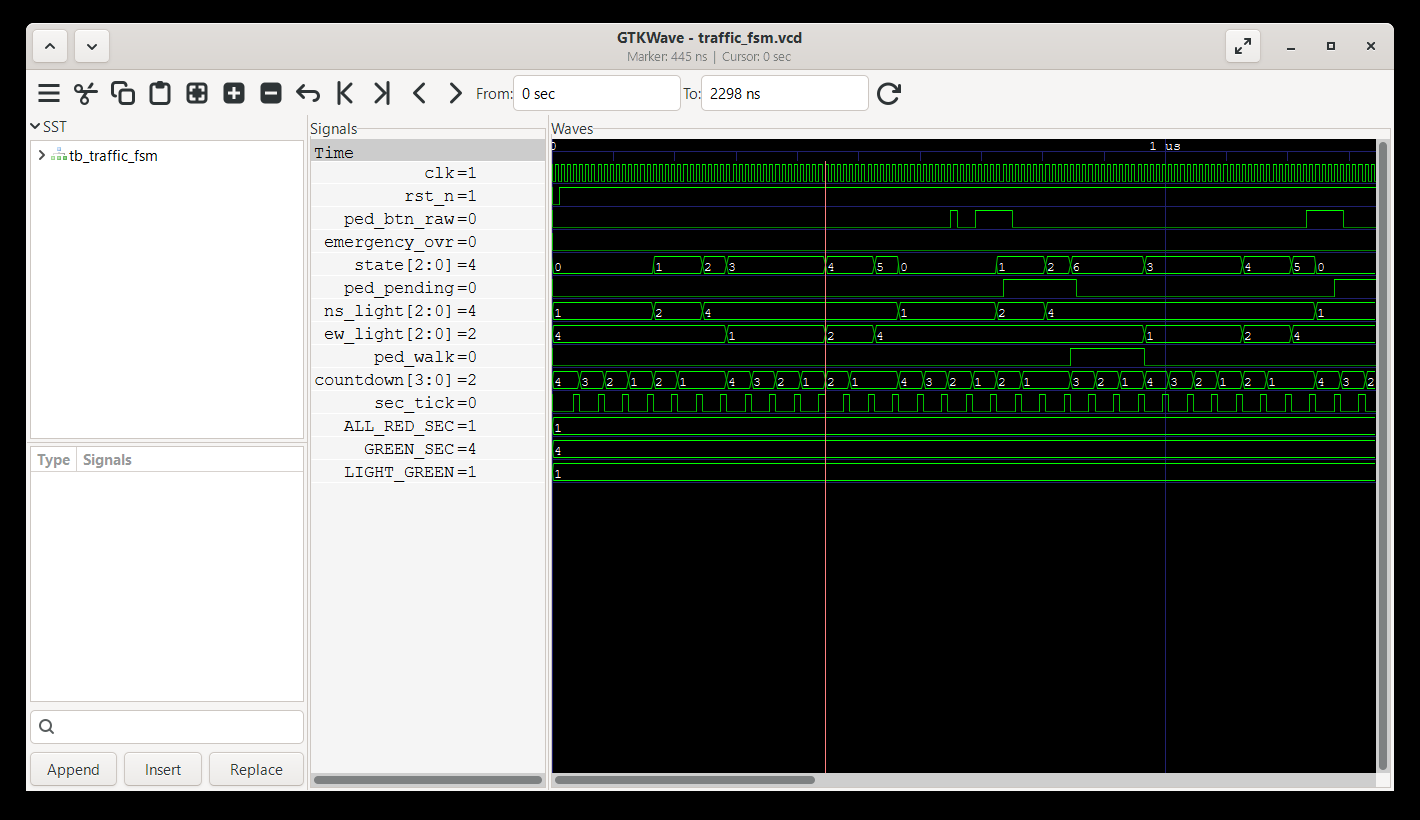
\includegraphics[width=0.95\textwidth,height=0.40\textheight,keepaspectratio]{figures/fig_0_gtkwave_waveform.png}
    \caption{GTKWave Verified Simulation Waveform (traffic\_fsm) — 638 transition columns audited.}
\end{figure}

\begin{figure}[H]
    \centering
    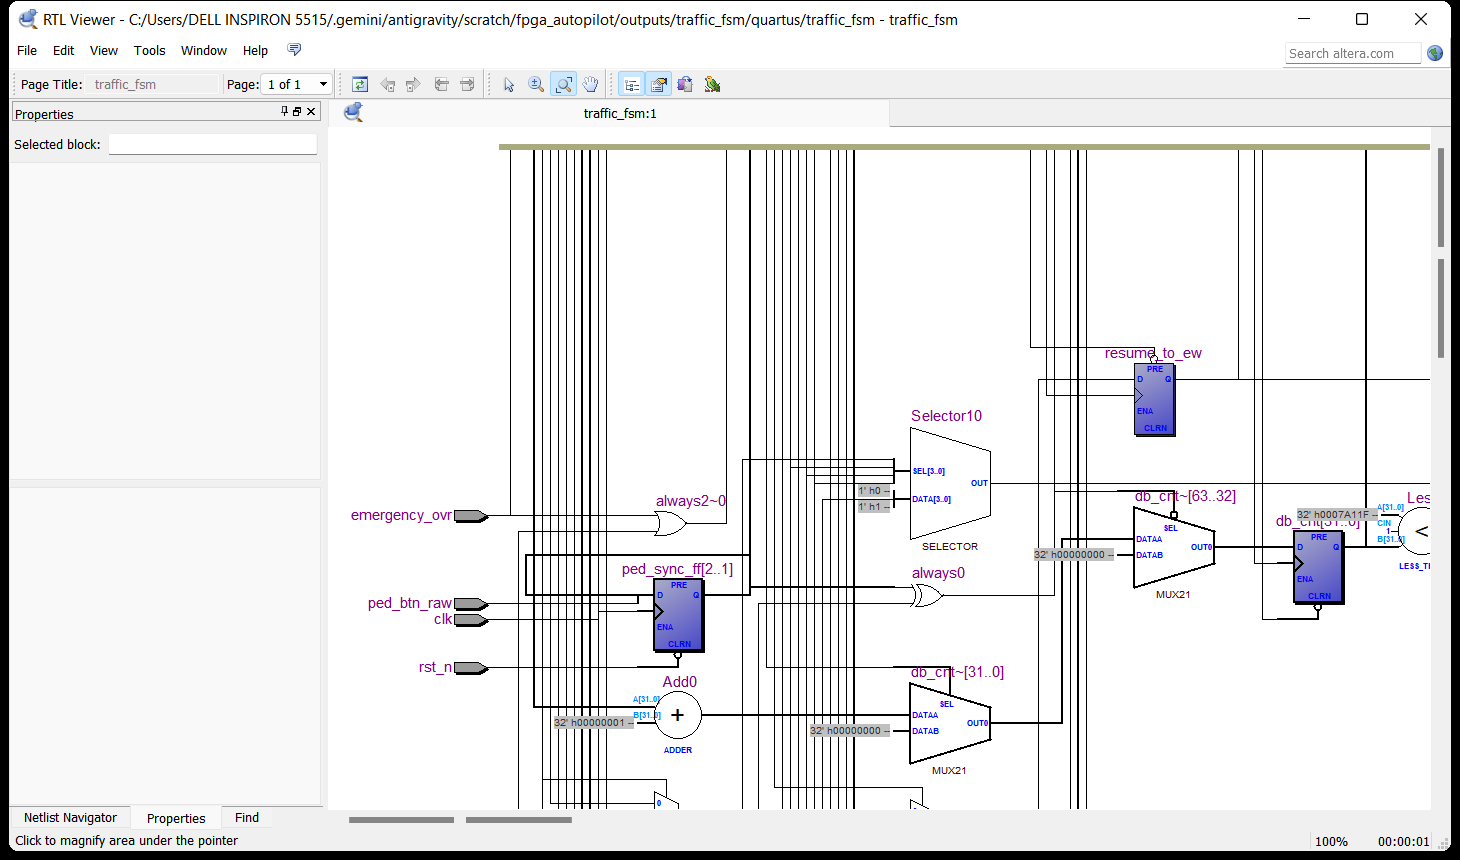
\includegraphics[width=0.95\textwidth,height=0.40\textheight,keepaspectratio]{figures/fig_1_quartus_rtl_viewer.png}
    \caption{Quartus II RTL Viewer Synthesized Schematic (traffic\_fsm).}
\end{figure}

\begin{figure}[H]
    \centering
    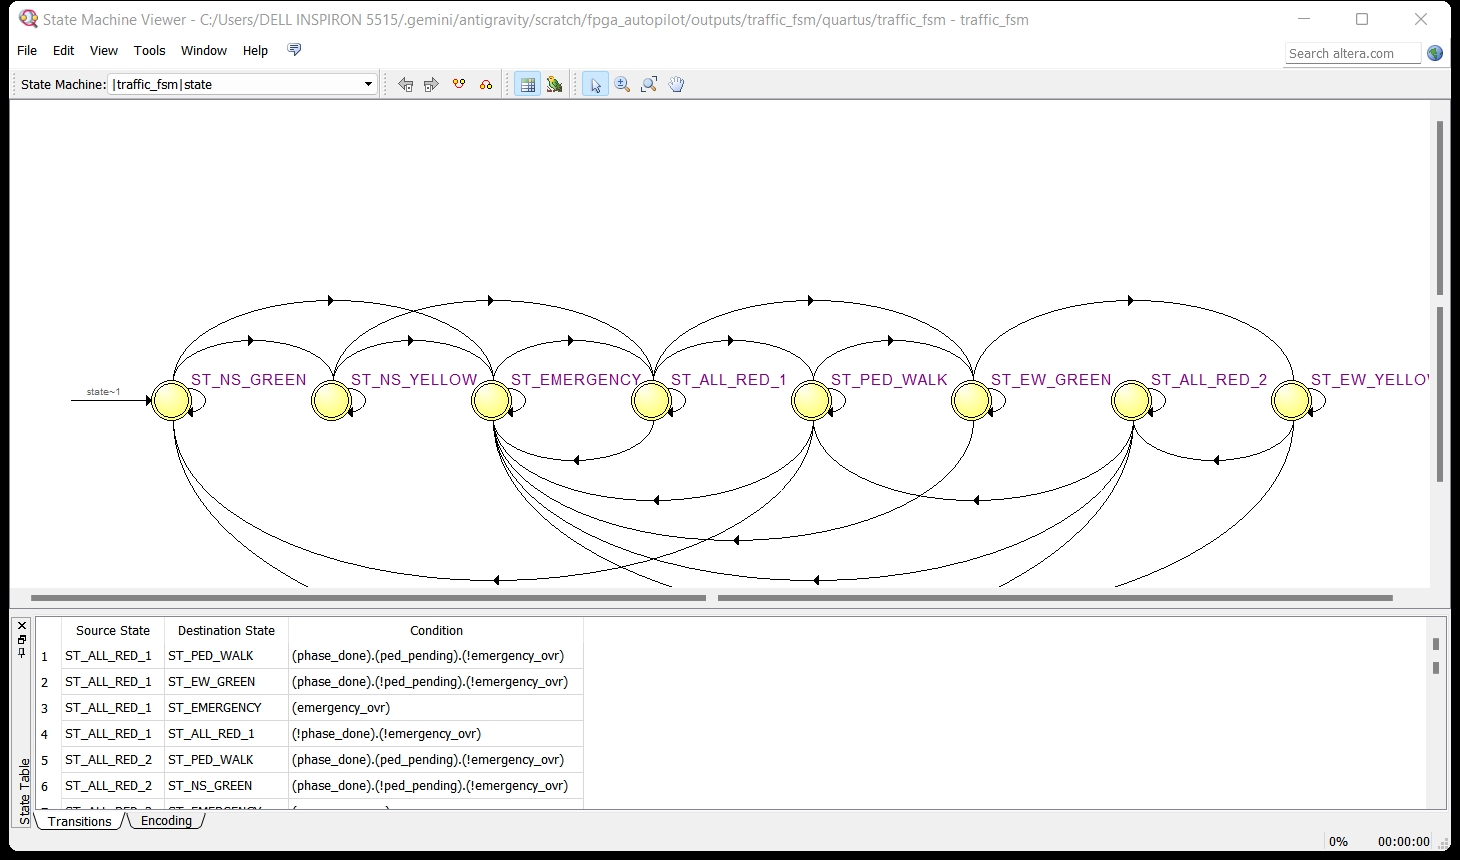
\includegraphics[width=0.95\textwidth,height=0.40\textheight,keepaspectratio]{figures/fig_2_quartus_fsm_viewer.png}
    \caption{Quartus II State Machine Viewer Diagram (traffic\_fsm).}
\end{figure}


\end{document}
